\frametitle{Mephenytoin}
\begin{columns}
\begin{column}{0.6\linewidth}
	\par Mephenytoin (C$_{12}$H$_{14}$N$_{2}$O$_{2}$, Mesantoin) is an antiepileptic drug with a heterocyclic organic compound.
	Structure of mephenytoin is an imidazolidine-2,4-dione (hydantoin) in which the imidazolidine nucleus carries a methyl group at N-3 and has ethyl and phenyl substituents at C-5, respectively.
	Mechanism of action is, promotes sodium efflux from neurons in motor cortex, and stabilizes the threshold against hyperexcitability caused by excessive stimulation.
	Due to these properties, mephenytoin reduces the membrane sodium gradient and prevents cortical seizure signal spreading.
	The 3D structure of Mephenytoin obtained from ZINC database with code 453.
\end{column}
\begin{column}{0.4\linewidth}
	\begin{figure}
		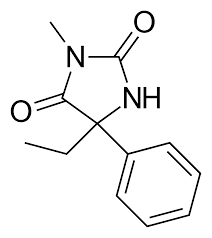
\includegraphics[width=0.8\linewidth]{mephenytoin_str.png}
		\caption{\centering The structure of Mephenytoin.}
		\label{fig:mph_structure}
	\end{figure}
\end{column}
\end{columns}